\section{Test on Monte Carlo}
\label{sec:MCTrial}

The alignment of the \lhcb RICH optical system was tested on simulated events.
The procedure described was applied to simulated events generated with a
misaligned optical system. \Fig{fig:RICHMCTest}
\begin{figure}[hbtp]
  \vspace*{-0.5\baselineskip}
  \centering
  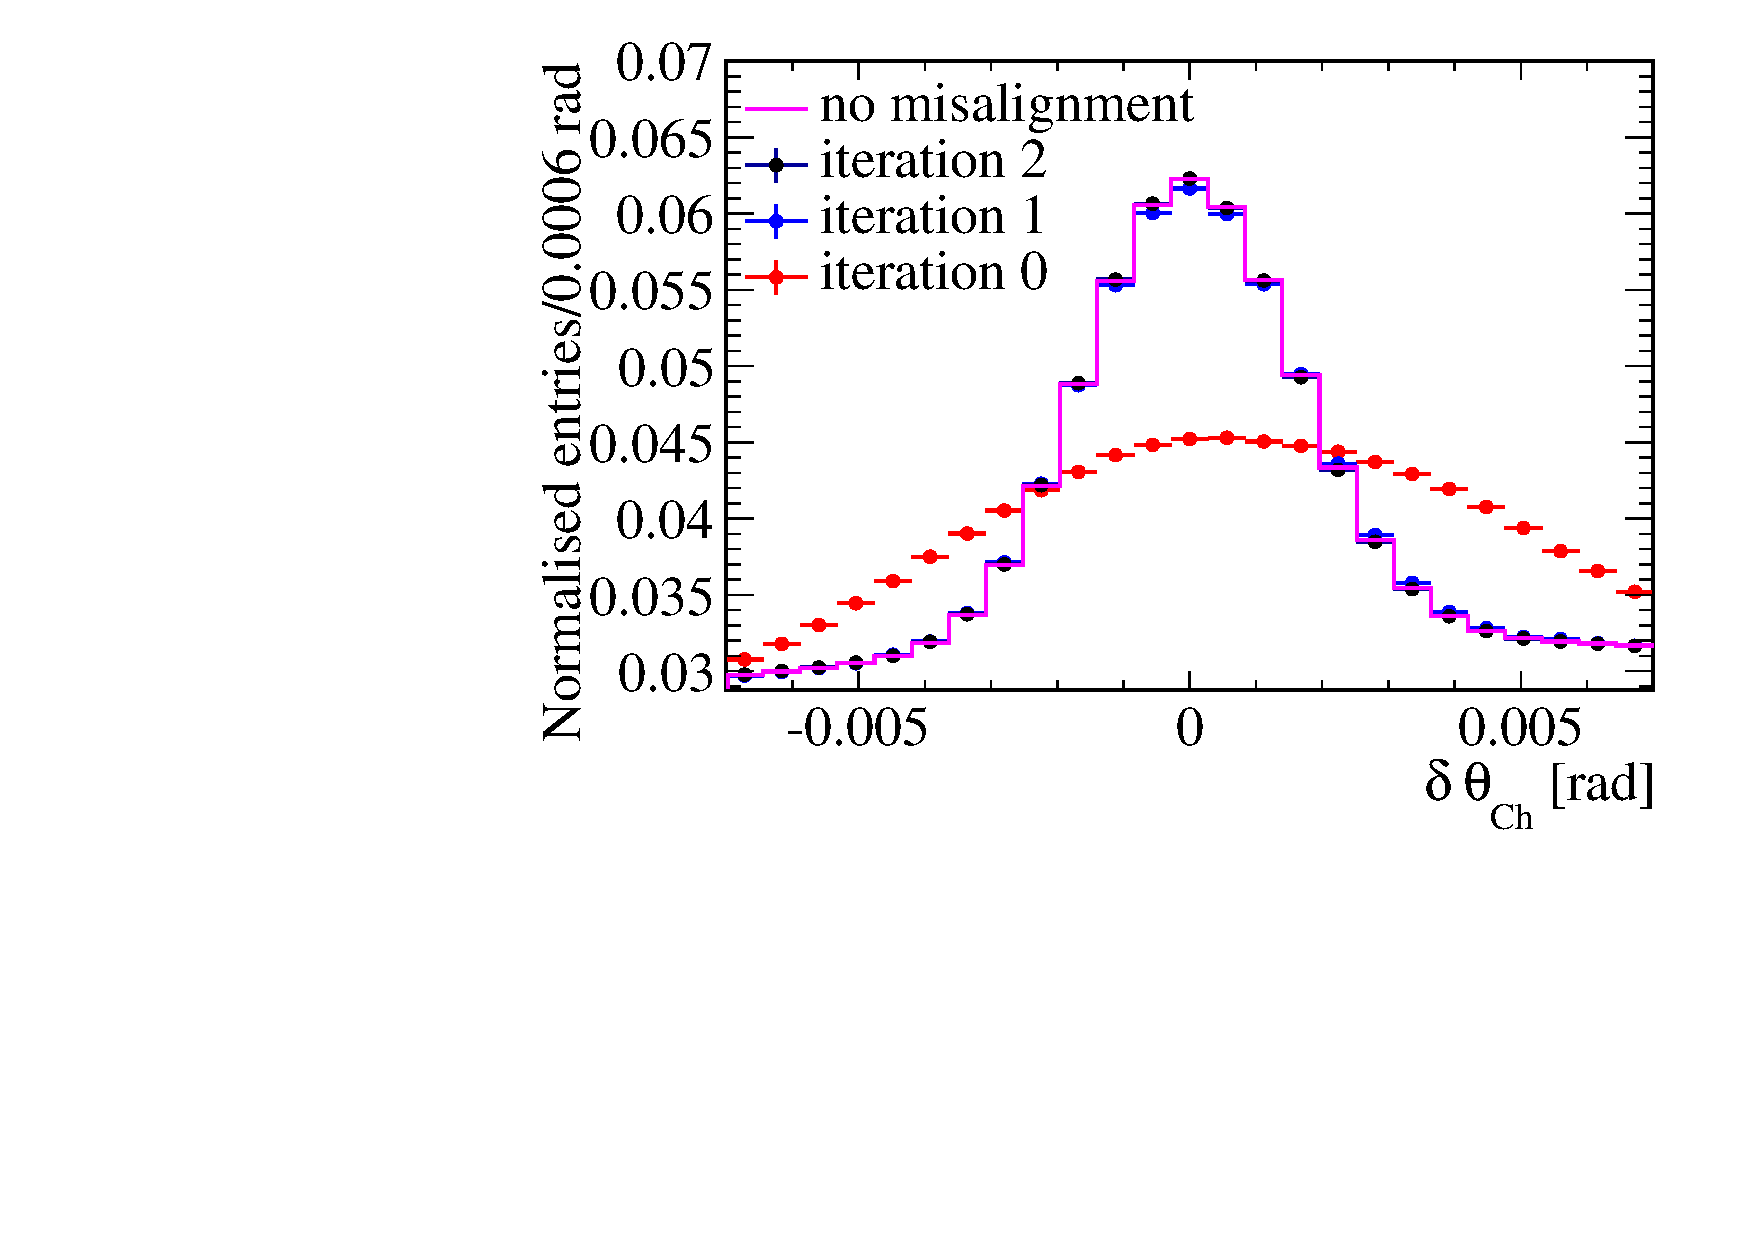
\includegraphics[width=0.49\textwidth, height=0.35\textwidth]
                  {figs/Results/RICH1_Alignment_MC10.pdf}
  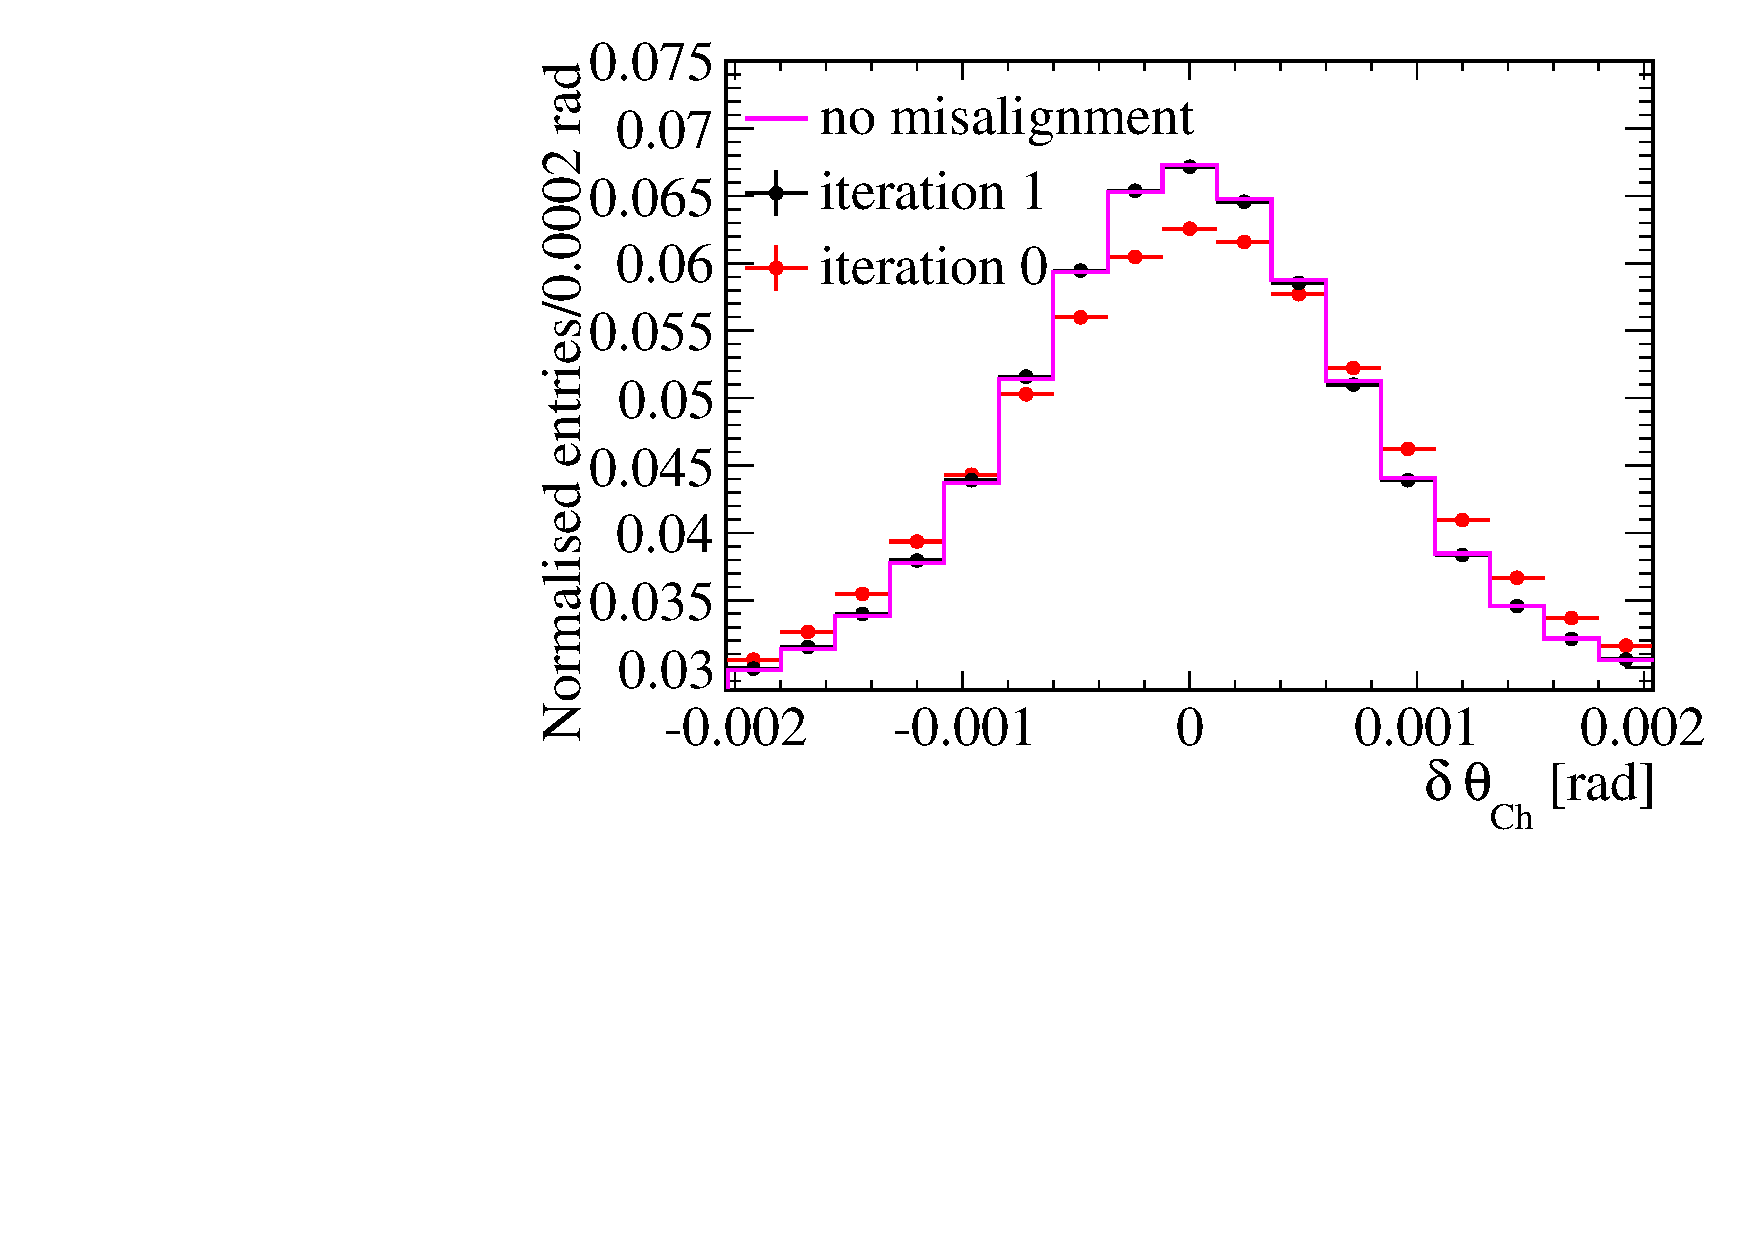
\includegraphics[width=0.49\textwidth, height=0.35\textwidth]
                  {figs/Results/RICH2_Alignment_MC10.pdf}
  \vspace*{-0.9\baselineskip}
  \caption{
    \deltatheta distribution for each iteration of the alignment procedure
    applied to misaligned Monte Carlo simulated data. Results are shown for the
    \richone detector (left) and the \richtwo  detector (right).}
  \label{fig:RICHMCTest}
  \vspace*{-0.5\baselineskip}
\end{figure}
shows the Cherenkov angle distribution for both RICH detectors after each
iteration of the alignment procedure, starting with the simulated misaligned
case. The results of this alignment are compared to those from simulated events
with a perfectly aligned system. Before convergence, each iteration of the
optical alignment procedure results in the distribution becoming closer to that
of the perfectly aligned case. The standard deviation of the \deltatheta
distribution for the RICH1 detector improves from $6.02\pm 0.04\mrad$ to
$1.563\pm 0.002\mrad$. Whereas for the \richtwo detector the resolution improves
from $0.772\pm 0.001\mrad$ in the misaligned case to  $0.668\pm 0.001\mrad$
after the alignment. The standard deviation for a perfectly aligned
\richone/\richtwo optical system is found to be  $1.569\pm
0.007\mrad$/$0.687\pm 0.003\mrad$.


\section{Alignment results}
\label{sec:AlignmentResults}

The alignment system presented here has been used throughout \lhcb data taking
since it began in 2010. The results shown here are from 2011 data applied to the
B\,hadron stream, using Stripping\,17 and Reco\,12. \deltatheta is plotted for
each iteration of the alignment process in~\fig{fig:RICHresolutionResults}.
\begin{figure}[hbtp]
  \vspace*{-0.5\baselineskip}
  \centering
  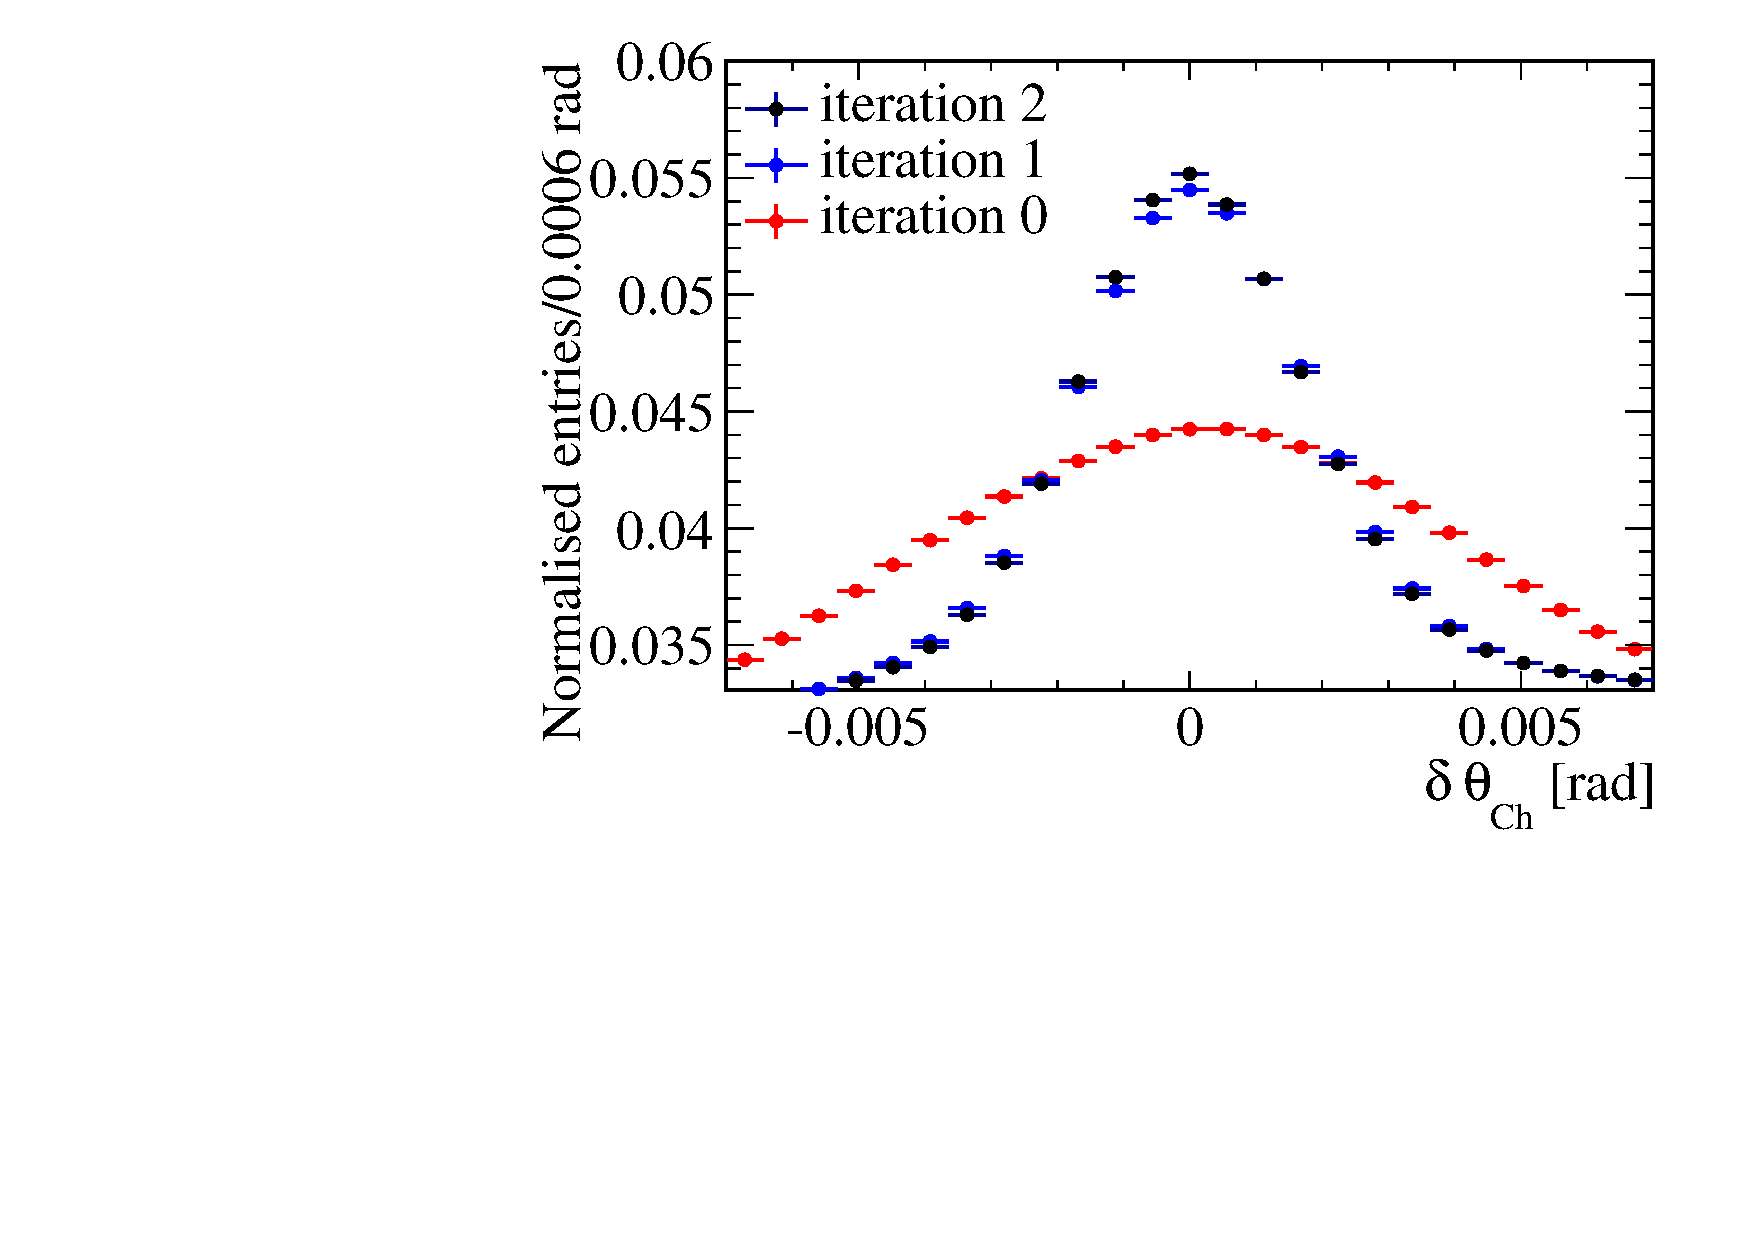
\includegraphics[width=0.49\textwidth]{figs/Results/RICH1_Alignment_2011.pdf}
  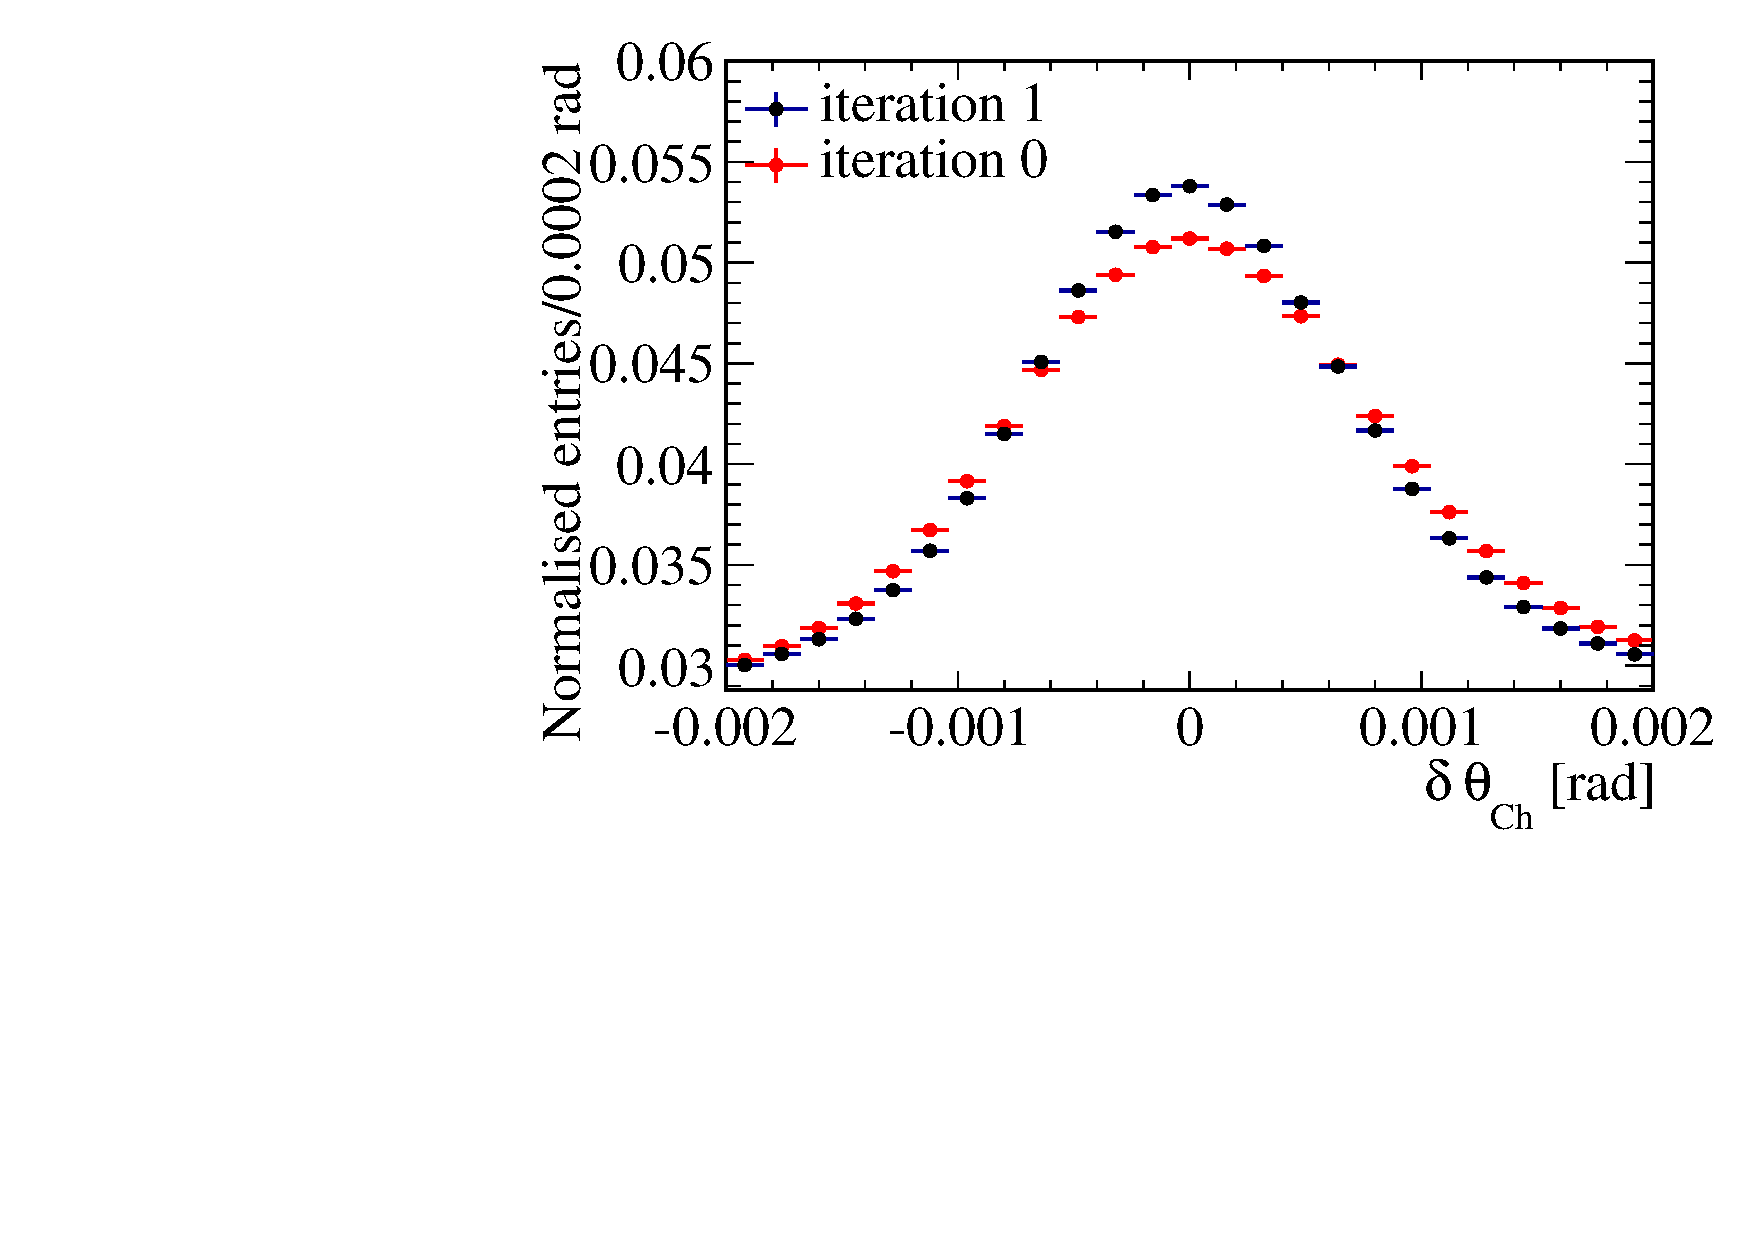
\includegraphics[width=0.49\textwidth]{figs/Results/RICH2_Alignment_2011.pdf}
  \vspace*{-0.9\baselineskip}
  \caption{
    \deltatheta is plotted for each iteration in the alignment of the \lhcb RICH
    optical system. \richone is shown on the left and \richtwo on the right. 
    Iteration 0 shows the \deltatheta distribution for the RICH detector with no
    software corrections for misalignments in the optical system. Corrections
    are then applied at each iteration until each mirror has a misalignment less
    than $0.1\mrad$ at which point the system is said to be aligned.}
  \label{fig:RICHresolutionResults}
  \vspace*{-0.5\baselineskip}
\end{figure}
Iteration~0 shows the resolution of the RICH detectors with no software
corrections for misalignments each subsequent iteration results in the
distribution getting closer to that of a perfectly aligned system.

Two iterations are required to align the mirrors of \richone from a state where
no corrections are assumed to an aligned state. Only a single pass is required
to align the optical system of the \richtwo detector. The extra iteration
required by the alignment procedure for \richone is believed to be due to the
initial conditions being much further than those for the aligned state.

The standard deviation of the \deltatheta distribution for \richone/\richtwo
without corrections (iteration 0) is $13.96\pm 0.05\mrad$/$0.73\pm
0.001\mrad$. This is improved to $1.602\pm 0.003\mrad$/$0.638\pm 0.0003\mrad$
after aligning the optical system of the RICH detectors, and compares to
$1.569\pm 0.007\mrad$/$0.687\pm 0.003\mrad$ for the perfectly aligned
\richone/\richtwo system.

The software alignment procedure for the \lhcb RICH mirrors has significantly
improved the resolution of both RICH detectors. However, the resolution  of the
\richone detector does not yet match that expected from simulation. There could
be many reasons for this including effects from the magnetic field.


\section{Conclusion} \label{sec:conclusions}

A method for alignment of the optical system of the \lhcb RICH detector
consisting of two sets of mirror segments installed in radiator vessels was
developed and presented. The developed method was tested with simulated events
and applied to data collected at the \lhcb experiment. The optical system is
aligned to within $0.1\mrad$, at which point the error due to mirror
misalignment becomes a small contribution.


\section{Acknowledgments} \label{sec:acknowledgments}

We are are grateful to Antonis Papanestis (RAL) for acquainting us with his
progress towards solving the problem of mirror alignment, to Chris Jones
(Cambridge) for photon reconstruction implementation, to all members of the
\lhcb RICH group and to Jonas Rademacker (University of Bristol) for numerous
discussions and consultations. Also we appreciate assistance of the \ganga team,
\lhcb core software group, Stefan Roisier (LCG group, CERN) and Lorenzo Moneta
(\root group, CERN).
